\section{Reproducible numerical comparisons}\label{sec:experiments}
\subsection{Analytical controls retained from the initial study}
The fixed controls use \eqref{eq:exp_family} with
$R\in\{1,2,4,6,8\}$, $A\in\{1,1000\}$, start $(R,0)$, and
$\varepsilon=10^{-6}$. Both short-step methods use \eqref{eq:stop}
with $\gamma=1$. Gap-log uses $L_0=L_1=1$ and Global-$L$ uses the
smallest uniform bound $L=e^R$. The choices of $A$ give identical
trajectories, not independent instances. Table~\ref{tab:endpoint}
includes the endpoint comparators needed to interpret this control.
\begin{table}[ht]
\centering
\caption{Updates on the exponential control. The last column follows
from the oracle returning the minimizer. A terminal point query
certifies termination.}\label{tab:endpoint}
\begin{tabular}{rrrr}
\toprule
$R$ & Gap-log & Global-$L$ & Open-loop / exact line search\\
\midrule
1 & 2 & 1 & 1\\
2 & 5 & 6 & 1\\
4 & 17 & 52 & 1\\
6 & 35 & 400 & 1\\
8 & 60 & 2976 & 1\\
\bottomrule
\end{tabular}
\end{table}
Four further controls use \eqref{eq:nonconvex}, $f(x)=x+x^2/2$
on $[0,1]$ from $1$, $f(x)=x$ on the same interval from $1$, and
\eqref{eq:exp_family} with $R=4,A=1000$ starting at $(0,0)$.
They take $5,1,1,0$ updates. All 24 historical runs pass the original
checks. Their summary values reproduce; some trajectory entries differ
in the last floating-point digits across environments. No cross-platform
byte identity of numerical traces is claimed.

\subsection{Protocol for multidimensional regression}
We use \eqref{eq:poisson} over Euclidean balls. For
$n\in\{4,12\}$ and seeds $11,29,47$, draw $m=12n$ independent
standard Gaussian rows and normalize each to unit Euclidean norm.
Draw a further Gaussian vector and scale its norm to $1.2$; call it
$b$. Generate integer counts $y_i\sim\operatorname{Poisson}(e^{a_i^Tb})$.
Use radii $R\in\{0.5,2,4\}$ and starts $0,Re_1,-Re_1$.
The six datasets, three radii and three starts give 18 constrained
problems and 54 starting configurations. Radii and starts sharing data
are dependent conditions, not independent statistical samples.

All methods use \eqref{eq:stop}, $\gamma=1$, $\varepsilon=10^{-4}$,
and a cap of 20,000 outer attempts. Parameters are fixed in
\texttt{Code/benchmark\_multidim.py} and written to the protocol file
before execution. The matrices and counts are saved.
Proposition~\ref{prop:poisson} supplies gap and norm parameters;
\eqref{eq:poisson_uniform} supplies the uniform bound.
These bounds are not tuned after observing performance.

Eight rules are compared. Gap-log uses \eqref{eq:log_step};
Global-$L$ uses $\min\{1,G/(L\|d\|^2)\}$; Open-loop uses $2/(k+2)$.
Armijo starts at $1$ and halves until \eqref{eq:armijo} holds.
Backtracking uses the quadratic-model test of~\cite{pedregosa},
with initial estimate $M=1$, per-iteration initial trial $M/2$,
and doubling on failure. Norm-based uses
$\min\{1,G/[e(K_0+K_1\|\nabla f\|)\|d\|^2]\}$ from~\cite{vyguzov}.
Line bisection checks the endpoint derivative, then bisects a
sign-changing bracket to width $10^{-12}$; it approximates exact
line search. AC-FW implements Algorithms~1--2 and damping (6),
with $\delta=1$, of~\cite{acfw}; its compulsory initial LMO move is
charged and may increase the objective. The implementations are
independent of the cited authors' software.

Function, full-gradient and LMO counters increment on every actual call.
Rejected function trials and gradients used in bisection are counted.
Accepted function values are reused; after an AC rejection the unchanged
gradient and atom are reused. No solver receives an optimum.
Separately, SLSQP gives a diagnostic interval $[f(z)-G(z),f(z)]$;
its largest computed width is $2.75\cdot10^{-7}$.
Seven of the 18 reference solutions are on the boundary and eleven
are interior according to the recorded tolerance. These are
floating-point diagnostics, not exact optimality proofs.

\subsection{Results and computational costs}
There are 432 recorded solver runs. Gap-log and six other methods
converge in all 54 configurations; Open-loop reaches the cap in nine,
all with $n=4,R=4$. The unfinished final certificates range from
$1.07\cdot10^{-4}$ to $1.80\cdot10^{-4}$ and remain in all summaries.
Table~\ref{tab:costs} reports medians over all 54 configurations,
including capped endpoints. The costs of a capped method must not
be interpreted as guaranteed costs to convergence.

\begin{table}[ht]
\centering\small
\caption{Recorded costs: successes, updates $N$, function calls $F$,
gradient calls $H$, LMO calls $V$, and milliseconds.
Time is first the median of three sequential untraced repetitions
per configuration, then the median across configurations;
validation and file output are excluded.}\label{tab:costs}
\begin{tabular}{lrrrrrr}
\toprule
Rule & Success & $N$ & $F$ & $H$ & $V$ & ms\\
\midrule
\csname @@input\endcsname multidim_table.tex
\bottomrule
\end{tabular}
\end{table}

\begin{table}[ht]
\centering\small
\caption{Median recorded updates at each radius, across 18 starting
configurations. All capped Open-loop runs belong to $R=4$.}
\label{tab:radius}
\begin{tabular}{lrrr}
\toprule
Rule & $R=0.5$ & $R=2$ & $R=4$\\
\midrule
\csname @@input\endcsname radius_table.tex
\bottomrule
\end{tabular}
\end{table}

At $R=4$, Gap-log improves on the supplied uniform bound in median
updates (216.5 versus 819), whereas the uniform rule is cheaper at
the two smaller radii. Backtracking and AC-FW are substantially cheaper
than Gap-log on this collection. Armijo uses fewer gradients and LMOs
but pays for repeated function trials; line bisection uses many gradients.
Separating oracle types changes the interpretation of update counts.
The experiment supports limitations of a fixed global bound in some
regimes, but not superiority over adaptive alternatives.

\begin{figure}[ht]
\centering
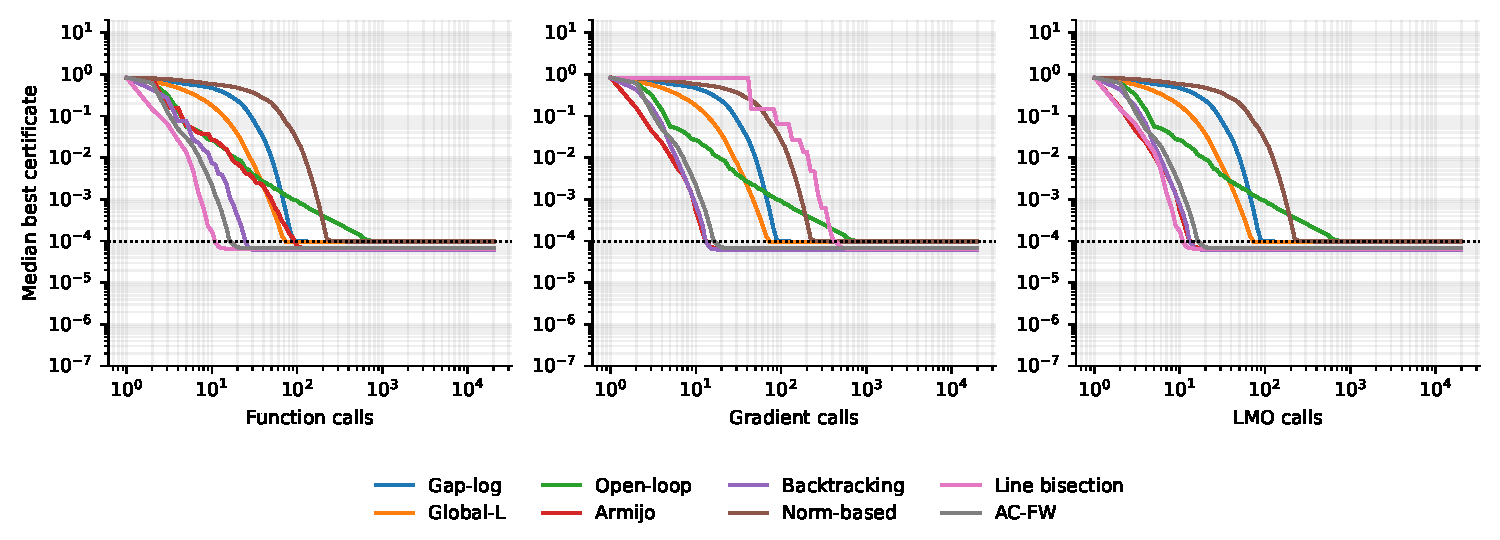
\includegraphics[width=\linewidth]{figures/multidim_en.pdf}
\caption{Median best recorded certificate versus separate oracle budgets
over the same 54 configurations. Values after termination or the run cap
are held at the last best recorded value. The dotted line is $10^{-4}$.
The panels use different cost units, which are not added together.}
\label{fig:cost_curves}
\end{figure}

\paragraph{Reproduction and validation.}
\texttt{Code/benchmark\_gap.py} reproduces the historical controls;
\texttt{Code/benchmark\_multidim.py} records multidimensional iterates,
parameters, statuses and counters.
\texttt{Code/report\_results.py} generates tables and figures from saved
data without solving new problems.
The trace audit checks feasibility, lower-bound consistency with the
diagnostic intervals, applicable descent and step bounds, and oracle
accounting on 340,433 recorded points. Hessian bounds are sampled at
up to 25 points per run; their global justification is
Proposition~\ref{prop:poisson}, not this sampling.
Eight separate tests check derivatives by finite differences, the scalar
inequality, scaling, actual interface calls, initial stopping, Armijo
trials, bisection and a nonoptimal oracle endpoint.
The 13 historical symbolic identities also pass.
Dependencies and commands are included in the accompanying archive.
